\documentclass[hyperref, a4paper]{article}

\usepackage{geometry}
\usepackage{titling}
\usepackage{titlesec}
% No longer needed, since we will use enumitem package
% \usepackage{paralist}
\usepackage{enumitem}
\usepackage{footnote}
\usepackage{enumerate}
\usepackage{amsmath, amssymb, amsthm}
\usepackage{mathtools}
\usepackage{bbm}
\usepackage{cite}
\usepackage{graphicx}
\usepackage{subfigure}
\usepackage{physics}
\usepackage{tensor}
\usepackage{siunitx}
\usepackage{slashed}
\usepackage{centernot}
\usepackage[version=4]{mhchem}
\usepackage{tikz}
\usepackage{xcolor}
\usepackage{listings}
\usepackage{autobreak}
\usepackage[ruled, vlined, linesnumbered]{algorithm2e}
\usepackage{nameref,zref-xr}
\zxrsetup{toltxlabel}
\zexternaldocument*[hw2-]{../2/2}[2.pdf]
\usepackage[colorlinks,unicode]{hyperref} % , linkcolor=black, anchorcolor=black, citecolor=black, urlcolor=black, filecolor=black
\usepackage[most]{tcolorbox}
\usepackage{prettyref}

% Page style
\geometry{left=3.18cm,right=3.18cm,top=2.54cm,bottom=2.54cm}
\titlespacing{\paragraph}{0pt}{1pt}{10pt}[20pt]
\setlength{\droptitle}{-5em}
\preauthor{\vspace{-10pt}\begin{center}}
\postauthor{\par\end{center}}

% More compact lists 
\setlist[itemize]{
    itemindent=17pt, 
    leftmargin=1pt,
    listparindent=\parindent,
    parsep=0pt,
}

% Math operators
\DeclareMathOperator{\timeorder}{\mathcal{T}}
\DeclareMathOperator{\diag}{diag}
\DeclareMathOperator{\legpoly}{P}
\DeclareMathOperator{\primevalue}{P}
\DeclareMathOperator{\sgn}{sgn}
\newcommand*{\ii}{\mathrm{i}}
\newcommand*{\ee}{\mathrm{e}}
\newcommand*{\const}{\mathrm{const}}
\newcommand*{\suchthat}{\quad \text{s.t.} \quad}
\newcommand*{\argmin}{\arg\min}
\newcommand*{\argmax}{\arg\max}
\newcommand*{\normalorder}[1]{: #1 :}
\newcommand*{\pair}[1]{\langle #1 \rangle}
\newcommand*{\fd}[1]{\mathcal{D} #1}
\DeclareMathOperator{\bigO}{\mathcal{O}}

% Feynman slash
\newcommand{\fsl}[1]{{\centernot{#1}}}

% TikZ setting
\usetikzlibrary{arrows,shapes,positioning}
\usetikzlibrary{arrows.meta}
\usetikzlibrary{decorations.markings}
\tikzstyle arrowstyle=[scale=1]
\tikzstyle directed=[postaction={decorate,decoration={markings,
    mark=at position .5 with {\arrow[arrowstyle]{stealth}}}}]
\tikzstyle ray=[directed, thick]
\tikzstyle dot=[anchor=base,fill,circle,inner sep=1pt]

% Algorithm setting
% Julia-style code
\SetKwIF{If}{ElseIf}{Else}{if}{}{elseif}{else}{end}
\SetKwFor{For}{for}{}{end}
\SetKwFor{While}{while}{}{end}
\SetKwProg{Function}{function}{}{end}
\SetArgSty{textnormal}

\newcommand*{\concept}[1]{{\textbf{#1}}}

% Embedded codes
\lstset{basicstyle=\ttfamily,
  showstringspaces=false,
  commentstyle=\color{gray},
  keywordstyle=\color{blue}
}

% Reference formatting
\newrefformat{fig}{Figure~\ref{#1} on page~\pageref{#1}}

% Color boxes
\tcbuselibrary{skins, breakable, theorems}
\newtcbtheorem[number within=section]{warning}{Warning}%
  {colback=orange!5,colframe=orange!65,fonttitle=\bfseries, breakable}{warn}
\newtcbtheorem[number within=section]{note}{Note}%
  {colback=green!5,colframe=green!65,fonttitle=\bfseries, breakable}{note}
\newtcbtheorem[number within=section]{info}{Info}%
  {colback=blue!5,colframe=blue!65,fonttitle=\bfseries, breakable}{info}

\newcommand{\hwtwo}{\href{../2/2.pdf}{Homework 2}}

\title{QFT I, Homework 5}
\author{Jinyuan Wu}

\begin{document}

\maketitle

\paragraph{Gordon identity} Derive the Gordon identity [problem $3.2$ on p. 72 of Peskin],
\begin{equation}
    \bar{u}\left(p^{\prime}\right) \gamma^{\mu} u(p)=\bar{u}\left(p^{\prime}\right)\left[\frac{p^{\prime \mu}+p^{\mu}}{2 m}+\frac{i \sigma^{\mu \nu} q_{\nu}}{2 m}\right] u(p),
    \label{eq:gordon-id}
\end{equation}
where $q=\left(p^{\prime}-p\right)$. We will put this formula to use in Chapter 6 .

\paragraph{Solution} Since we have Eq.~(3.22) in Peskin
\begin{equation}
    \acomm*{\gamma^\mu}{\gamma^\nu} = 2 \eta^{\mu \nu}, 
\end{equation}
and 
\begin{equation}
    \frac{1}{2} \comm*{\gamma^\mu}{\gamma^\nu} = - \ii \sigma^{\mu \nu}
\end{equation}
in the beginning of Section~3.4 in Peskin, the RHS of \eqref{eq:gordon-id} is 
\[
    \begin{aligned}
        &\quad \bar{u}\left(p^{\prime}\right)\left[\frac{p^{\prime \mu}+p^{\mu}}{2 m}+\frac{\ii \sigma^{\mu \nu} q_{\nu}}{2 m}\right] u(p) \\
        &= \frac{1}{2m} \bar{u}\left(p^{\prime}\right) ( (p' + p)_\nu \eta^{\mu \nu} + \ii \sigma^{\mu \nu} (p' - p)_\nu ) u(p) \\
        &= \frac{1}{2m} \bar{u}(p') \left( \frac{1}{2} \acomm*{\gamma^\mu}{\gamma^\nu} (p' + p)_\nu - \frac{1}{2} \comm*{\gamma^\mu}{\gamma^\nu} (p' - p)_\nu \right) u(p).
    \end{aligned}
\]
Expanding the last line, we have 
\[
    \frac{1}{2} \acomm*{\gamma^\mu}{\gamma^\nu} (p' + p)_\nu - \frac{1}{2} \comm*{\gamma^\mu}{\gamma^\nu} (p' - p)_\nu = \gamma^\mu \gamma^\nu p_\nu + \gamma^\nu \gamma^\mu p'_\nu,
\]
and therefore by using the Dirac equation 
\[
    (\gamma^\mu p_\mu - m) u(p) = 0, \quad \bar{u}(p) (\gamma^\mu p_\mu - m) = 0,
\]
we have
\[
    \begin{aligned}
        &\quad \frac{1}{2m} \bar{u}(p') \left( \frac{1}{2} \acomm*{\gamma^\mu}{\gamma^\nu} (p' + p)_\nu - \frac{1}{2} \comm*{\gamma^\mu}{\gamma^\nu} (p' - p)_\nu \right) u(p) \\
        &= \frac{1}{2m} \bar{u}(p') (\gamma^\mu \gamma^\nu p_\nu + p'_\nu \gamma^\nu \gamma^\mu ) u(p) \\
        &= \frac{1}{2m} (\bar{u}(p') \gamma^\mu m u(p) + \bar{u}(p') m \gamma^\mu u(p) ) = \text{LHS},
    \end{aligned}
\]
which is \eqref{eq:gordon-id}.

\paragraph{}

\paragraph{Rutherford scattering} [Problem $4.4$ on p. 129 of Peskin.] The cross section for scattering of an electron by the Coulomb field of a nucleus can be computed, to lowest order, without quantizing the electromagnetic field. Instead, treat the field as a given, classical potential $A_{\mu}(x)$. The interaction Hamiltonian is
\begin{equation}
    H_{I}=\int d^{3} x e \bar{\psi} \gamma^{\mu} \psi A_{\mu},
    \label{eq:interaction-ham-2}
\end{equation}
where $\psi(x)$ is the usual quantized Dirac field.
(a) Show that the $T$-matrix element for electron scattering off a localized classical potential is, to lowest order,
\[
\left\langle p^{\prime}|i T| p\right\rangle=-i e \bar{u}\left(p^{\prime}\right) \gamma^{\mu} u(p) \cdot \tilde{A}_{\mu}\left(p^{\prime}-p\right)
\]
where $\widetilde{A}_{\mu}(q)$ is the four-dimensional Fourier transform of $A_{\mu}(x)$.
(b) If $A_{\mu}(x)$ is time independent, its Fourier transform contains a delta function of energy. It is then natural to define
\[
\left\langle p^{\prime}|i T| p\right\rangle=i \mathcal{M} \cdot(2 \pi) \delta\left(E_{f}-E_{i}\right)
\]
where $E_{i}$ and $E_{f}$ are the initial and final energies of the particle, and to adopt a new Feynman rule for computing $\mathcal{M}$ :
\begin{equation}
    \begin{gathered}
        \begin{tikzpicture}[x=0.75pt,y=0.75pt,yscale=-0.75,xscale=0.75]
            %uncomment if require: \path (0,300); %set diagram left start at 0, and has height of 300
            
            %Straight Lines [id:da21043242361216352] 
            \draw    (163,181.25) -- (193,124.92) ;
            \draw [shift={(178,153.08)}, rotate = 118.04] [fill={rgb, 255:red, 0; green, 0; blue, 0 }  ][line width=0.08]  [draw opacity=0] (12,-3) -- (0,0) -- (12,3) -- cycle    ;
            %Straight Lines [id:da6825093279600336] 
            \draw    (168,171.67) -- (158,190.83) ;
            
            %Straight Lines [id:da2766305483503835] 
            \draw    (188,115.25) -- (158,58.92) ;
            \draw [shift={(173,87.08)}, rotate = 61.96] [fill={rgb, 255:red, 0; green, 0; blue, 0 }  ][line width=0.08]  [draw opacity=0] (12,-3) -- (0,0) -- (12,3) -- cycle    ;
            %Straight Lines [id:da7541746616043725] 
            \draw    (183,105.67) -- (193,124.83) ;
            
            %Straight Lines [id:da6302347302021725] 
            \draw    (193,125) .. controls (194.67,123.33) and (196.33,123.33) .. (198,125) .. controls (199.67,126.67) and (201.33,126.67) .. (203,125) .. controls (204.67,123.33) and (206.33,123.33) .. (208,125) .. controls (209.67,126.67) and (211.33,126.67) .. (213,125) .. controls (214.67,123.33) and (216.33,123.33) .. (218,125) .. controls (219.67,126.67) and (221.33,126.67) .. (223,125) .. controls (224.67,123.33) and (226.33,123.33) .. (228,125) .. controls (229.67,126.67) and (231.33,126.67) .. (233,125) .. controls (234.67,123.33) and (236.33,123.33) .. (238,125) .. controls (239.67,126.67) and (241.33,126.67) .. (243,125) .. controls (244.67,123.33) and (246.33,123.33) .. (248,125) .. controls (249.67,126.67) and (251.33,126.67) .. (253,125) .. controls (254.67,123.33) and (256.33,123.33) .. (258,125) .. controls (259.67,126.67) and (261.33,126.67) .. (263,125) .. controls (264.67,123.33) and (266.33,123.33) .. (268,125) -- (271,125) -- (271,125) ;
            %Flowchart: Summing Junction [id:dp8906099185423473] 
            \draw   (271,125) .. controls (271,119.71) and (275.29,115.42) .. (280.58,115.42) .. controls (285.88,115.42) and (290.17,119.71) .. (290.17,125) .. controls (290.17,130.29) and (285.88,134.58) .. (280.58,134.58) .. controls (275.29,134.58) and (271,130.29) .. (271,125) -- cycle ; \draw   (273.81,118.22) -- (287.36,131.78) ; \draw   (287.36,118.22) -- (273.81,131.78) ;
            \end{tikzpicture}            
    \end{gathered}=- \ii e \gamma^{\mu} \tilde{A}_{\mu}(\vb*{q})
\end{equation}
where $\widetilde{A}_{\mu}(q)$ is the three-dimensional Fourier transform of $A_{\mu}(x)$. Given this definition of $\mathcal{M}$, show that the cross section for scattering off a time independent, localized potential is
\begin{equation}
    d \sigma=\frac{1}{v_{i}} \frac{1}{2 E_{i}(2 \pi)^{3}} \frac{d^{3} p_{f}}{2 E_{f}}\left|\mathcal{M}\left(p_{i} \rightarrow p_{f}\right)\right|^{2}(2 \pi) \delta\left(E_{f}-E_{i}\right)
    \label{eq:single-cross-section}
\end{equation}
where $v_{i}$ is the particle's initial velocity. This formula is a natural modification of (4.79). Integrate over $\left|p_{f}\right|$ to find a simple expression for $d \sigma / d \Omega$.
(c) pecialize to the case of electron scattering from a Coulomb potential $\left(A^{0}=\right.$ $Z e / 4 \pi r)$. Working in the nonrelativistic limit, derive the Rutherford formula,
\begin{equation}
    \frac{d \sigma}{d \Omega}=\frac{\alpha^{2} Z^{2}}{4 m^{2} v^{4} \sin ^{4}(\theta / 2)}.
    \label{eq:rutherford}
\end{equation}
(With a few calculational tricks from Section 5.1, you will have no difficulty evaluating the general cross section in the relativistic case; see Problem 5.1.)

\paragraph{Solution} \begin{itemize}
\item[(a)] We work in the interaction picture. The leading order is 
\[
    \begin{aligned}
        \mel{p', s'}{ 1 + \ii T }{p, s} &= 1 - \ii \int_{-\infty}^\infty \dd{t} \mel{p', s'}{H_\text{I}}{p, s} \\
        &= 1 - \ii e \int_{-\infty}^\infty \dd{t} \int \dd[3]{\vb*{x}} \mel{p', s'}{\bar{\psi} \gamma^{\mu} \psi A_{\mu}}{p, s} + \cdots \\
        &= 1 - \ii e \int \dd[4]{x} \mel{0}{ \sqrt{2 E_{\vb*{p}'}} a_{\vb*{p}'}^{s'} \bar{\psi} \gamma^{\mu} \psi A_{\mu} \sqrt{2 E_{\vb*{p}}} a^{s\dagger}_{\vb*{p}} }{0} + \cdots.
    \end{aligned}
\] 
The expansions of $\psi, \bar{\psi}$ (Peskin Eq.~(3.99) and (3.100)) are 
\[
    \begin{aligned}
        \psi(x) &= \int \frac{\dd[3]{\vb*{p}}}{(2\pi)^3} \frac{1}{\sqrt{2 E_{\vb*{p}}}} \sum_s \left( a^s_{\vb*{p}} u^s(p) \ee^{- \ii p \cdot x} + b_{\vb*{p}}^{s\dagger} v^s(p) \ee^{\ii p \cdot x} \right), \\
        \bar{\psi}(x) &= \int \frac{\dd[3]{\vb*{p}}}{(2\pi)^3} \frac{1}{\sqrt{2 E_{\vb*{p}}}} \sum_s \left( a^{s \dagger}_{\vb*{p}} \bar{u}^s(p) \ee^{\ii p \cdot x} + b_{\vb*{p}}^{s} \bar{v}^s(p) \ee^{- \ii p \cdot x} \right) ,
    \end{aligned}
\]
and we expand the electric field as 
\[
    A_\mu(x) = \int \frac{\dd[4]{k}}{(2\pi)^4} \tilde{A}_\mu(k) \ee{- \ii k \cdot x},
\]
so we have 
\[
    \begin{aligned}
        &\quad - \ii e \int \dd[4]{x} \mel{0}{ \sqrt{2 E_{\vb*{p}'}} a_{\vb*{p}'}^{s'} \bar{\psi} \gamma^{\mu} \psi A_{\mu} \sqrt{2 E_{\vb*{p}}} a^{s\dagger}_{\vb*{p}} }{0} \\
        &= - \ii e \sqrt{2 E_{\vb*{p}}} \sqrt{2 E_{\vb*{p}'}} \int \dd[4]{x} \int \frac{\dd[3]{\vb*{q}'}}{(2\pi)^3} \int \frac{\dd[3]{\vb*{q}}}{(2\pi)^3} \int \frac{\dd[4]{k}}{(2\pi)^4} \frac{1}{\sqrt{2 E_{\vb*{q}}}} \frac{1}{\sqrt{2 E_{\vb*{q}'}}} \sum_{\sigma, \sigma'} \bra{0} a^{s'}_{\vb*{p}'} ( a^{\sigma' \dagger}_{\vb*{q}'} \bar{u}^{\sigma'}(q') \ee^{\ii q' \cdot x} \\
        &\quad \quad + b^{\sigma'}_{\vb*{q}'} \bar{v}^{\sigma'}(q') \ee^{- \ii q' \cdot x} ) \gamma^\mu ( a^\sigma_{\vb*{q}} u^\sigma(q) \ee^{- \ii q \cdot x} + b^{\sigma \dagger}_{\vb*{q}} v^\sigma(q) \ee^{\ii q \cdot x} ) 
        \tilde{A}_\mu(k) \ee^{- \ii k \cdot x} a^{s \dagger}_{\vb*{p}} \ket{0} \\
        &= - \ii e \sqrt{2 E_{\vb*{p}}} \sqrt{2 E_{\vb*{p}'}} \int \frac{\dd[3]{\vb*{q}'}}{(2\pi)^3} \int \frac{\dd[3]{\vb*{q}}}{(2\pi)^3} \int \frac{\dd[4]{k}}{(2\pi)^4} \frac{1}{\sqrt{2 E_{\vb*{q}}}} \frac{1}{\sqrt{2 E_{\vb*{q}'}}} \sum_{\sigma, \sigma'} \bra{0} a^{s'}_{\vb*{p}'} \times \\
        & \quad \quad ( (2\pi)^4 \delta^4(q'-q-k) a^{\sigma' \dagger}_{\vb*{q}'} a^\sigma_{\vb*{q}} \bar{u}^{\sigma'}(q') \gamma^\mu u^\sigma(q) \tilde{A}_\mu(k) + (2\pi)^4 \delta^4(-q' - q +k) b^{\sigma'}_{\vb*{q}'} a^\sigma_{\vb*{q}} \bar{v}^{\sigma'}(q') \gamma^\mu u^\sigma(q) \tilde{A}_\mu (k) \\
        &\quad \quad + (2\pi)^4 \delta^4(q' + q - k) a^{\sigma' \dagger}_{\vb*{q}'} b^{\sigma \dagger}_{\vb*{q}} \bar{u}^{\sigma'}(q') \gamma^\mu v^\sigma(q) \tilde{A}_\mu(k) + 
        (2\pi)^4 \delta^4(-q' + q - k) b^{\sigma'}_{\vb*{q}'} b^{\sigma \dagger}_{\vb*{q}} \bar{v}^{\sigma'}(q') \gamma^\mu v^\sigma(q) \tilde{A}_\mu(k) ) a^{s \dagger}_{\vb*{p}} \ket*{0}.
    \end{aligned}
\]
We can then integrate out $k$ and replace the $k$ in $\tilde{A}_\mu(k)$ with $q$ and $q'$.
By Wick theorem, the second and the third term vanish because a antiparticle cannot be automatically transformed
into a particle, and vice versa. The operators in the first term contract into 
\[
    \mel{0}{a^{s'}_{\vb*{p}'} a^{\sigma' \dagger}_{\vb*{q}'} a^\sigma_{\vb*{q}} a^{s \dagger}_{\vb*{p}} }{0} = (2\pi)^3 \delta^{s \sigma} \delta^3(\vb*{p} - \vb*{q}) \times (2\pi)^3 \delta^{s' \sigma'} \delta^3(\vb*{p}' - \vb*{q}'),
\]
and the operators in the fourth term contract into 
\[
    \mel{0}{a^{s'}_{\vb*{p}'} b^{\sigma'}_{\vb*{q}'} b^{\sigma \dagger}_{\vb*{q}} a^{s \dagger}_{\vb*{p}} }{0} = (2\pi)^3 \delta^{s s'} \delta^3(\vb*{p} - \vb*{p}') \times (2\pi)^3 \delta^{\sigma \sigma'} \delta^3(\vb*{q} - \vb*{q}').
\]
Therefore we have
\[
    \begin{aligned}
        &\quad - \ii e \int \dd[4]{x} \mel{0}{ \sqrt{2 E_{\vb*{p}'}} a_{\vb*{p}'}^{s'} \bar{\psi} \gamma^{\mu} \psi A_{\mu} \sqrt{2 E_{\vb*{p}}} a^{s\dagger}_{\vb*{p}} }{0} \\
        &= - \ii e \bar{u}^{s'}(p') \gamma^\mu u^s(p) \tilde{A}_\mu(p' - p) - \ii e \bar{v}^{\sigma'} \gamma^\mu v^\sigma(p) \tilde{A}_\mu(0) (2\pi)^3 \delta^3(0) \delta^3(\vb*{p} - \vb*{p}'). 
    \end{aligned}
\]
Since the potential is localized, there is no such thing as a uniform field present at every point in the world, 
and therefore $A_\mu(0) = 0$. So finally we get a first-order approximation of the transition matrix:
\begin{equation}
    \mel{p', s'}{\ii T}{p, s} = - \ii e \bar{u}^{s'}(p') \gamma^\mu u^s(p) \tilde{A}_\mu(p' - p) ,
\end{equation}
or in the matrix form, 
\begin{equation}
    \mel{p'}{\ii T}{p} = - \ii e \bar{u}(p') \gamma^\mu u(p) \tilde{A}_\mu(p' - p).
\end{equation}

\item[(b)] In this case, we have 
\begin{equation}
    A_\mu(k) = \int \dd[4]{x} \ee^{\ii k \cdot x} A_\mu(\vb*{x}) = 2 \pi \delta(k^0) \int \dd[3]{\vb*{x}} \ee^{- \ii \vb*{k} \cdot \vb*{x}} A_\mu(\vb*{x}) = 2 \pi \delta(k^0) A_\mu(\vb*{k}). 
\end{equation}  
Therefore, 
\begin{equation}
    \begin{aligned}
        \mel{p'}{\ii T}{p} &= - \ii e \bar{u}(p') \gamma^\mu u(p) 2 \pi \delta(E_{\vb*{p}'} - E_{\vb*{p}}) A_\mu(\vb*{k}) \\
        &= \ii \mathcal{M} \cdot (2\pi) \delta(E_f - E_i) ,
    \end{aligned}
\end{equation}
where
\begin{equation}
    \ii \mathcal{M} = - \ii e \bar{u}(p') \gamma^\mu u(p) A_\mu(\vb*{k}).
\end{equation}

The formula \eqref{eq:single-cross-section} can be seen as a specific case of Eq.~(4.79). 
We consider \eqref{eq:interaction-ham-2} to be an effective theory around the state in which there is one heavy
particle, and the electric charge density and current density of it are stable and happen to generate an 
electromagnetic field $A^\mu$. By taking the inverse of the Maxwell equation and design the wave function of 
the heavy particle carefully, we can always make this happen. We call \eqref{eq:interaction-ham-2} the
``effective'' theory and call the theory with a heavy field the ``original'' theory. 
Diagrammatically, what we are doing is \begin{equation}
    \begin{gathered}
        \begin{tikzpicture}[x=0.75pt,y=0.75pt,yscale=-1,xscale=1]
            %uncomment if require: \path (0,300); %set diagram left start at 0, and has height of 300
            
            %Straight Lines [id:da2072677508539662] 
            \draw    (340,198.63) -- (370,142.29) ;
            \draw [shift={(355,170.46)}, rotate = 118.04] [fill={rgb, 255:red, 0; green, 0; blue, 0 }  ][line width=0.08]  [draw opacity=0] (12,-3) -- (0,0) -- (12,3) -- cycle    ;
            %Straight Lines [id:da0222576558033718] 
            \draw    (345,189.04) -- (335,208.21) ;
            
            %Straight Lines [id:da6933200630259788] 
            \draw    (365,132.63) -- (335,76.29) ;
            \draw [shift={(350,104.46)}, rotate = 61.96] [fill={rgb, 255:red, 0; green, 0; blue, 0 }  ][line width=0.08]  [draw opacity=0] (12,-3) -- (0,0) -- (12,3) -- cycle    ;
            %Straight Lines [id:da8416418921744453] 
            \draw    (360,123.04) -- (370,142.21) ;
            
            %Straight Lines [id:da47437638161561635] 
            \draw    (370,142.38) .. controls (371.67,140.71) and (373.33,140.71) .. (375,142.38) .. controls (376.67,144.05) and (378.33,144.05) .. (380,142.38) .. controls (381.67,140.71) and (383.33,140.71) .. (385,142.38) .. controls (386.67,144.05) and (388.33,144.05) .. (390,142.38) .. controls (391.67,140.71) and (393.33,140.71) .. (395,142.38) .. controls (396.67,144.05) and (398.33,144.05) .. (400,142.38) .. controls (401.67,140.71) and (403.33,140.71) .. (405,142.38) .. controls (406.67,144.05) and (408.33,144.05) .. (410,142.38) .. controls (411.67,140.71) and (413.33,140.71) .. (415,142.38) .. controls (416.67,144.05) and (418.33,144.05) .. (420,142.38) .. controls (421.67,140.71) and (423.33,140.71) .. (425,142.38) -- (426,142.38) -- (426,142.38) ;
            %Flowchart: Summing Junction [id:dp14723461604231702] 
            \draw   (426,142.38) .. controls (426,137.08) and (430.29,132.79) .. (435.58,132.79) .. controls (440.88,132.79) and (445.17,137.08) .. (445.17,142.38) .. controls (445.17,147.67) and (440.88,151.96) .. (435.58,151.96) .. controls (430.29,151.96) and (426,147.67) .. (426,142.38) -- cycle ; \draw   (428.81,135.6) -- (442.36,149.15) ; \draw   (442.36,135.6) -- (428.81,149.15) ;
            
            %Straight Lines [id:da7269240022160504] 
            \draw    (95,198.5) -- (125,142.17) ;
            \draw [shift={(110,170.33)}, rotate = 118.04] [fill={rgb, 255:red, 0; green, 0; blue, 0 }  ][line width=0.08]  [draw opacity=0] (12,-3) -- (0,0) -- (12,3) -- cycle    ;
            %Straight Lines [id:da08518637836608556] 
            \draw    (100,188.92) -- (90,208.08) ;
            
            %Straight Lines [id:da9058585014851037] 
            \draw    (120,132.5) -- (90,76.17) ;
            \draw [shift={(105,104.33)}, rotate = 61.96] [fill={rgb, 255:red, 0; green, 0; blue, 0 }  ][line width=0.08]  [draw opacity=0] (12,-3) -- (0,0) -- (12,3) -- cycle    ;
            %Straight Lines [id:da03151163576845506] 
            \draw    (115,122.92) -- (125,142.08) ;
            
            %Straight Lines [id:da9524401068957293] 
            \draw    (125,142.25) .. controls (126.67,140.58) and (128.33,140.58) .. (130,142.25) .. controls (131.67,143.92) and (133.33,143.92) .. (135,142.25) .. controls (136.67,140.58) and (138.33,140.58) .. (140,142.25) .. controls (141.67,143.92) and (143.33,143.92) .. (145,142.25) .. controls (146.67,140.58) and (148.33,140.58) .. (150,142.25) .. controls (151.67,143.92) and (153.33,143.92) .. (155,142.25) .. controls (156.67,140.58) and (158.33,140.58) .. (160,142.25) .. controls (161.67,143.92) and (163.33,143.92) .. (165,142.25) .. controls (166.67,140.58) and (168.33,140.58) .. (170,142.25) .. controls (171.67,143.92) and (173.33,143.92) .. (175,142.25) .. controls (176.67,140.58) and (178.33,140.58) .. (180,142.25) .. controls (181.67,143.92) and (183.33,143.92) .. (185,142.25) -- (187,142.25) -- (187,142.25) ;
            %Straight Lines [id:da4183958705248685] 
            \draw [line width=2.25]    (187,72.92) -- (187,211.58) ;
            %Straight Lines [id:da6432897133746458] 
            \draw    (187,122.25) -- (187,100.92) ;
            \draw [shift={(187,98.92)}, rotate = 90] [fill={rgb, 255:red, 0; green, 0; blue, 0 }  ][line width=0.08]  [draw opacity=0] (12,-3) -- (0,0) -- (12,3) -- cycle    ;
            %Straight Lines [id:da8943747483436242] 
            \draw    (187,193.25) -- (187,171.92) ;
            \draw [shift={(187,169.92)}, rotate = 90] [fill={rgb, 255:red, 0; green, 0; blue, 0 }  ][line width=0.08]  [draw opacity=0] (12,-3) -- (0,0) -- (12,3) -- cycle    ;
            
            
            % Text Node
            \draw (250,134.65) node [anchor=north west][inner sep=0.75pt]    {$\simeq $};
            % Text Node
            \draw (115,238.67) node [anchor=north west][inner sep=0.75pt]   [align=left] {original};
            % Text Node
            \draw (358,238.67) node [anchor=north west][inner sep=0.75pt]   [align=left] {effective};
            % Text Node
            \draw (92,72.77) node [anchor=south west] [inner sep=0.75pt]    {$p'$};
            % Text Node
            \draw (92,211.48) node [anchor=north west][inner sep=0.75pt]    {$p$};
            % Text Node
            \draw (156,138.85) node [anchor=south] [inner sep=0.75pt]    {$k$};
            % Text Node
            \draw (398,138.98) node [anchor=south] [inner sep=0.75pt]    {$k$};
            % Text Node
            \draw (337,72.89) node [anchor=south west] [inner sep=0.75pt]    {$p'$};
            % Text Node
            \draw (337,211.61) node [anchor=north west][inner sep=0.75pt]    {$p$};
            % Text Node
            \draw (189,72.92) node [anchor=west] [inner sep=0.75pt]    {$q'$};
            % Text Node
            \draw (189,211.58) node [anchor=west] [inner sep=0.75pt]    {$q$};
            \end{tikzpicture}   
    \end{gathered}     
    \label{eq:original-eff-eq}
\end{equation}
We can fix $q$ and $q'$ to two arbitrary values, as long as they are small enough (correct because the particle 
is heavy) and satisfy the conservation of momentum.

Under the basis of the original theory, we have 
\[
    \begin{aligned}
        \ii \mathcal{M}^\text{original} &= - \ii e \bar{u}(p') \gamma^\mu u(p) \frac{- \ii}{p^2} \eta_{\mu \nu}
        (- \ii e) \bar{u}(q') \gamma^\nu u(q) \\
        &= - \ii e \bar{u}(p') \gamma^\mu u(p) \frac{- 1}{p^2} \bar{u}(q') \gamma_\mu u(q) .
    \end{aligned}
\]
Since under the Lorenz gauge we have 
\[
    j^\mu = e \bar{\psi} \gamma^\mu \psi, \quad \partial_\mu \partial^\mu A^\nu = j^\mu,
\]
we find 
\[
    \expval*{A^\mu}(q - q') = - \frac{1}{p^2} \bar{u}(q') \gamma^\mu u(q).
\]
Under a mean field approximation, we can effectively write down 
\[
    \ii \mathcal{M}^\text{original} = - \ii e \bar{u}(p') \gamma^\mu u(p) A_\mu(q-  q'),
\]
which just looks like $\ii \mathcal{M}^\text{eff}$. However, note we have 
\[
    \ket*{p, \text{heavy particle}}_\text{origin} = \sqrt{2 E} \ket*{p}_\text{eff}, \quad 
    \ket*{p', \text{heavy particle}}_\text{origin} = \sqrt{2 E} \ket*{p'}_\text{eff},
\]
where $E$ is the energy of the heavy particle, which, since the particle is heavy, almost does not change. 
The $\sqrt{2 M}$ factors come from the fact that in relativistic QFT the covariant many-body wave 
function is defined as 
\[
    \ket*{p_1, p_2, \ldots, p_n} = \sqrt{2 E_{1}} a^\dagger_{\vb*{p}_1} \cdots \sqrt{2 E_n} a^\dagger_{\vb*{p}_n} \ket*{0},
\]
and $\ket*{p}_\text{eff}$ misses the factor for the heavy particle. Therefore, we have
\begin{equation}
    \mathcal{M}^\text{original} = 2 E \mathcal{M}^\text{eff} .
\end{equation} 
Factors like the $2E$ can also be seen when one switch from the $\ket*{p} = \sqrt{2 E_{\vb*{p}}} 
a^\dagger_{\vb*{p}} \ket*{0}$ basis to the $a^\dagger_{\vb*{p}} \ket*{0}$ basis, for example Eq.~(4.136) in Peskin.
Now Peskin (4.79) gives 
\[
    \begin{aligned}
        \dd{\sigma} &= \frac{1}{2 E_{\vb*{p}} 2 E \abs*{\vb*{v}_{\vb*{p}} - \vb*{v}_{\vb*{q}}}} 
        \frac{\dd[3]{\vb*{p}'}}{(2\pi)^3} \frac{1}{2 E_{\vb*{p}'}} \int \frac{\dd[3]{\vb*{q}'}}{(2\pi)^3} \frac{1}{2E} \abs*{\mathcal{M}^\text{origin}}^2 \\
        &\quad \quad \times (2\pi)^4 \delta(E_\text{f} + E - E_\text{i} - E) \delta^3(\vb*{q}' + \vb*{p}' - \vb*{q} - \vb*{p})  \\
        &= \frac{1}{2 E_{\vb*{p}} 2 E \abs*{\vb*{v}_{\vb*{p}}} } 
        \frac{\dd[3]{\vb*{p}'}}{(2\pi)^3} \frac{1}{2 E_{\vb*{p}'}} \int \frac{\dd[3]{\vb*{q}'}}{(2\pi)^3} \frac{1}{2E} \abs*{2 E \mathcal{M}^\text{eff}}^2 (2\pi)^4 \delta(E_{f} - E_{i} ) \delta^3(\vb*{q}' + \vb*{p}' - \vb*{q} - \vb*{p}) \\
        &= \frac{1}{v_{\vb*{p}}} \frac{1}{2 E_{\vb*{p}} (2\pi)^3} \frac{\dd[3]{\vb*{p}'}}{2 E_{\vb*{p}'}} \abs*{\mathcal{M}^\text{eff}}^2 (2\pi) \delta(E_f- E_i) ,
    \end{aligned}
\]
where the energy of the heavy particle does not change. Note that $\vb*{p}$ is the input momentum and $\vb*{p}'$
is the output momentum, and $\mathcal{M}^\text{eff}$ is just $\mathcal{M}$ in the context of 
\eqref{eq:interaction-ham-2}, and we find this is exactly \eqref{eq:single-cross-section}. 

Now we integrate $\abs*{\vb*{p}_f}$. We have (following the notation in Chapter 4 of Peskin, we use $\abs*{p_f}$ to denote $\abs*{\vb*{p}_f}^2$)
\[
    \begin{aligned}
        \dd{\sigma} &= \frac{1}{v_i} \frac{1}{2 E_i (2\pi)^3} \int \frac{ \abs*{{p}_f}^2 \dd{\Omega} \dd{\abs*{{p}_f}} }{2 E_f}
        \abs*{\mathcal{M}(p_i \to p_f)}^2 (2\pi) \delta(E_f - E_i) \\
        &= \frac{1}{v_i} \frac{1}{2 E_i (2\pi)^2} \eval{\frac{1}{{\abs*{p_f}}/{\sqrt{\abs*{p_f}^2 + m^2}}} \frac{\dd{\Omega} \abs*{p_f}^2}{2 E_i} \abs*{\mathcal{M}(p_i \to p_f)}^2}_{\sqrt{\abs*{p}_f^2 + m^2} = E_i} \\
        &= \frac{1}{v_i} \frac{1}{(2 E_i)^2 (2\pi)^2} \dd{\Omega} \abs*{p_f} E_i \abs*{\mathcal{M}(p_i \to p_f)}^2 \\
        &= \frac{1}{v_i} \frac{\dd{\Omega}}{16 \pi^2} \frac{\abs*{p_f}}{E_f} \abs*{\mathcal{M}(p_i \to p_f)}^2 \\
        &= \frac{\dd{\Omega}}{16 \pi^2} \abs*{\mathcal{M}(p_i \to p_f)}^2.
    \end{aligned}
\]
Therefore
\begin{equation}
    \dv{\sigma}{\Omega} = \frac{\abs*{\mathcal{M}(p_i \to p_f)}^2}{16 \pi^2}.
    \label{eq:cross-section-r-2}
\end{equation}

\item[(c)] For $A^0 = Ze / 4 \pi r$, we have the well-known Fourier transformation
\begin{equation}
    A^0(\vb*{q}) = \frac{Z e}{ \abs*{\vb*{q}}^2}.
    \label{eq:coulomb-point}
\end{equation}
We assume we are dealing with an averaged input spin, and in this case the $\abs{\mathcal{M}}^2$ in 
\eqref{eq:cross-section-r-2} should be replaced by $\frac{1}{2} \sum_\text{spin} \abs*{\mathcal{M}}^2$.

Note that $\gamma^0 \gamma^\mu$ is a Hermitian matrix, and we have (here we switch back to the notation 
of $p$ and $p'$ to keep agreement with Peskin's notation in Section~5.1) 
\[
    \begin{aligned}
        \sum_\text{spin} \abs*{\mathcal{M}}^2 &= e^2 \trace \bar{u}(p') \gamma^\mu \tilde{A}_\mu(p' - p) u(p) (\bar{u}(p') \gamma^\mu \tilde{A}_\mu(p' - p) u(p) )^\dagger \\
        &= e^2 \trace \bar{u}(p') \gamma^\mu \tilde{A}_\mu(p' - p) u(p) \bar{u}(p) \gamma^\nu \tilde{A}_\nu(p - p') u(p') \\
        &= e^2 \tilde{A}_\mu(p' - p) \tilde{A}_\nu(p - p') \trace u(p') \bar{u}(p') \gamma^\mu u(p) \bar{u}(p) \gamma^\nu \\
        &= e^2 \tilde{A}_\mu(p' - p) \tilde{A}_\nu(p - p') \trace (\fsl{p}' + m) \gamma^\mu (\fsl{p} + m) \gamma^\nu .
    \end{aligned}
\]
The second line can be justified in the discussion above Peskin Eq.~(5.2). The fourth line is because of Eq.~(5.3).
Now expanding the trace with $\gamma$ matrices trace formulae, we have 
\[
    \begin{aligned}
        &\quad \trace (\fsl{p}' + m) \gamma^\mu (\fsl{p} + m) \gamma^\nu \\
        &= \trace (p'_\rho p_\sigma \gamma^\rho \gamma^\mu \gamma^\sigma \gamma^\nu + m^2 \gamma^\mu \gamma^\nu + p'_\rho m \gamma^\rho \gamma^\mu \gamma^\nu + p_\sigma m \gamma^\mu \gamma^\sigma \gamma^\nu ) \\
        &= p'_\rho p_\sigma \times 4 (\eta^{\rho \mu} \eta^{\sigma \nu} - \eta^{\rho \sigma} \eta^{\mu \nu} + \eta^{\rho \nu} \eta^{\mu \sigma}) + m^2 \times 4 \eta^{\mu \nu} \\
        &= 4 (p'^\mu p^\nu + p'^\nu p^\mu - p'_\rho p^\rho \eta^{\mu \nu}) + 4 m^2 \eta^{\mu \nu},
    \end{aligned}
\]
and therefore 
\begin{equation}
    \begin{aligned}
        \sum_\text{spin} \abs*{\mathcal{M}}^2 &= e^2 \tilde{A}_\mu(p' - p) \tilde{A}_\nu(p - p') (4 (p'^\mu p^\nu + p'^\nu p^\mu - p'_\rho p^\rho \eta^{\mu \nu}) + 4 m^2 \eta^{\mu \nu}) \\
        &= 4 e^2 ( (\tilde{A}(p'-p) \cdot p') (\tilde{A}(p - p') \cdot p) + (\tilde{A}(p'-p) \cdot p) (\tilde{A}(p - p') \cdot p') \\
        &\quad \quad + (m^2 - p \cdot p') \tilde{A}(p'-p) \cdot \tilde{A}(p - p') ) .
    \end{aligned}
    \label{eq:general-m-2}
\end{equation}

From \eqref{eq:coulomb-point} we have 
\[
    A^0(p - p') = A^0(p' - p) = \frac{Ze}{ \abs*{\vb*{p} - \vb*{p}'}^2} = \frac{Ze}{ \left( 2 \abs*{\vb*{p}} \sin \frac{\theta}{2} \right)^2}, \quad A^i = 0.
\]
Substituting these into \eqref{eq:general-m-2}, we have 
\[
    \begin{aligned}
        \sum_\text{spin} \abs*{\mathcal{M}}^2 &= 4 e^2 \tilde{A}^0(p - p') \tilde{A}^0(p' - p) (2 p^0 p'^0 + (m^2 - p \cdot p') ) \\
        &= 4 e^2 \left( \frac{Ze}{ \left( 2 \abs*{\vb*{p}} \sin \frac{\theta}{2} \right)^2} \right)^2 (2 p^0 p'^0 + (m^2 - p^0 p'^0 + \vb*{p} \cdot \vb*{p}') ) \\
        &= \frac{(Z e^2)^2}{4 \abs*{\vb*{p}}^4 \sin^4 \frac{\theta}{2} } (E_{\vb*{p}}^2 + m^2 + \vb*{p} \cdot \vb*{p}') \\
        &= \frac{(Z e^2)^2}{4 \abs*{\vb*{p}}^4 \sin^4 \frac{\theta}{2} } (E_{\vb*{p}}^2 + E_{\vb*{p}}^2 - \abs*{\vb*{p}}^2 + \vb*{p} \cdot \vb*{p}') \\
        &= \frac{(Z e^2)^2}{4 \abs*{\vb*{p}}^2  \sin^4 \frac{\theta}{2} } ( \frac{2 E_{\vb*{p}}^2}{\abs*{\vb*{p}}^2} + \frac{- \abs*{\vb*{p}}^2 + \abs*{\vb*{p}}^2 \cos \theta }{\abs*{\vb*{p}}^2} ) \\
        &= \frac{(Z e^2)^2}{4 \abs*{\vb*{p}}^2 \sin^4 \frac{\theta}{2} } ( \frac{2}{v^2} + (\cos \theta - 1) ) \\
        &=  \frac{(Z e^2)^2}{4 \abs*{\vb*{p}}^2 \sin^4 \frac{\theta}{2} } \left( \frac{2}{v^2} - 2 \sin^2 \frac{\theta}{2} \right). 
    \end{aligned}
\]
Therefore we get 
\begin{equation}
    \dv{\sigma}{\Omega} = \frac{1}{16 \pi^2} \frac{1}{2} \sum_\text{spin} \abs*{\mathcal{M}}^2 = \frac{1}{16 \pi^2} \frac{(Z e^2)^2}{ 4 \abs*{\vb*{p}}^2 \sin^4 \frac{\theta}{2} } \left( \frac{1}{v^2} - \sin^2 \frac{\theta}{2} \right) = \frac{(Z \alpha)^2}{4 \abs*{\vb*{p}}^2 \sin^4 \frac{\theta}{2}} \left( \frac{1}{v^2} - \sin^2 \frac{\theta}{2} \right).
    \label{eq:relativistic-rutherford}
\end{equation}
\eqref{eq:relativistic-rutherford} is the relativistic cross section. In the non-relativistic limit, $v$ is small,
and $1 / v^2$ is dominantly large, and $\vb*{p} = mv$, so we have 
\begin{equation}
    \dv{\sigma}{\Omega} = \frac{(Z \alpha)^2}{ 4 m^2 v^4 \sin^4 \frac{\theta}{2} },
\end{equation}
which is just \eqref{eq:rutherford}.

\end{itemize}

\paragraph{}

\paragraph{Bhabha scattering} [Problem $5.2$ on p. 170 of Peskin.] Compute the differential cross section $d \sigma / d \cos \theta$ for Bhabha scattering, $e^{+} e^{-} \rightarrow e^{+} e^{-}$. You may work in the limit $E_{\mathrm{cm}} \gg m_{e}$, in which it is permissible to ignore the electron mass. There are two Feynman diagrams; these must be added in the invariant matrix element before squaring. Be sure that you have the correct relative sign between these diagrams. The intermediate steps are complicated, but the final result is quite simple. In particular, you may find it useful to introduce the Mandelstam variables $s, t$, and $u$. Note that, if we ignore the electron mass, $s+t+u=0$. You should be able to cast the differential cross section into the form
\begin{equation}
    \frac{d \sigma}{d \cos \theta}=\frac{\pi \alpha^{2}}{s}\left[u^{2}\left(\frac{1}{s}+\frac{1}{t}\right)^{2}+\left(\frac{t}{s}\right)^{2}+\left(\frac{s}{t}\right)^{2}\right].
    \label{eq:3-cross-section}
\end{equation}
Rewrite this formula in terms of $\cos \theta$ and graph it. What feature of the diagrams causes the differential cross section to diverge as $\theta \rightarrow 0$ ?

\paragraph{Solution} The diagrams are 
\begin{equation}
    \begin{gathered}
        \begin{tikzpicture}[x=0.75pt,y=0.75pt,yscale=-1,xscale=1]
            %uncomment if require: \path (0,300); %set diagram left start at 0, and has height of 300
            
            %Straight Lines [id:da11627769309979397] 
            \draw    (109,191.63) -- (139,135.29) ;
            \draw [shift={(124,163.46)}, rotate = 118.04] [fill={rgb, 255:red, 0; green, 0; blue, 0 }  ][line width=0.08]  [draw opacity=0] (12,-3) -- (0,0) -- (12,3) -- cycle    ;
            %Straight Lines [id:da0726415769300941] 
            \draw    (139,135.38) -- (103.58,201.58) ;
            
            %Straight Lines [id:da8619336144821805] 
            \draw    (134,125.63) -- (104,69.29) ;
            \draw [shift={(119,97.46)}, rotate = 61.96] [fill={rgb, 255:red, 0; green, 0; blue, 0 }  ][line width=0.08]  [draw opacity=0] (12,-3) -- (0,0) -- (12,3) -- cycle    ;
            %Straight Lines [id:da14762425357159215] 
            \draw    (129,116.04) -- (139,135.21) ;
            
            %Straight Lines [id:da25216137665038496] 
            \draw    (139,135.38) .. controls (140.67,133.71) and (142.33,133.71) .. (144,135.38) .. controls (145.67,137.05) and (147.33,137.05) .. (149,135.38) .. controls (150.67,133.71) and (152.33,133.71) .. (154,135.38) .. controls (155.67,137.05) and (157.33,137.05) .. (159,135.38) .. controls (160.67,133.71) and (162.33,133.71) .. (164,135.38) .. controls (165.67,137.05) and (167.33,137.05) .. (169,135.38) .. controls (170.67,133.71) and (172.33,133.71) .. (174,135.38) .. controls (175.67,137.05) and (177.33,137.05) .. (179,135.38) .. controls (180.67,133.71) and (182.33,133.71) .. (184,135.38) .. controls (185.67,137.05) and (187.33,137.05) .. (189,135.38) .. controls (190.67,133.71) and (192.33,133.71) .. (194,135.38) .. controls (195.67,137.05) and (197.33,137.05) .. (199,135.38) .. controls (200.67,133.71) and (202.33,133.71) .. (204,135.38) -- (207.58,135.38) -- (207.58,135.38) ;
            %Straight Lines [id:da8201615246277574] 
            \draw    (213,146.25) -- (243,202.58) ;
            \draw [shift={(228,174.42)}, rotate = 241.96] [fill={rgb, 255:red, 0; green, 0; blue, 0 }  ][line width=0.08]  [draw opacity=0] (12,-3) -- (0,0) -- (12,3) -- cycle    ;
            %Straight Lines [id:da45189740765819875] 
            \draw    (243,202.5) -- (207.58,136.29) ;
            
            %Straight Lines [id:da6431451523117473] 
            \draw    (236.58,79.88) -- (206.58,136.21) ;
            \draw [shift={(221.58,108.04)}, rotate = 298.04] [fill={rgb, 255:red, 0; green, 0; blue, 0 }  ][line width=0.08]  [draw opacity=0] (12,-3) -- (0,0) -- (12,3) -- cycle    ;
            %Straight Lines [id:da8092731448744368] 
            \draw    (231.58,89.46) -- (241.58,70.29) ;
            
            %Straight Lines [id:da7553877443671639] 
            \draw    (97,87) -- (119.02,125.93) ;
            \draw [shift={(120,127.67)}, rotate = 240.51] [fill={rgb, 255:red, 0; green, 0; blue, 0 }  ][line width=0.08]  [draw opacity=0] (12,-3) -- (0,0) -- (12,3) -- cycle    ;
            %Straight Lines [id:da9268251167261283] 
            \draw    (98,183.67) -- (120.02,144.74) ;
            \draw [shift={(121,143)}, rotate = 119.49] [fill={rgb, 255:red, 0; green, 0; blue, 0 }  ][line width=0.08]  [draw opacity=0] (12,-3) -- (0,0) -- (12,3) -- cycle    ;
            %Straight Lines [id:da5261940946788859] 
            \draw    (247.02,181.93) -- (225,143) ;
            \draw [shift={(248,183.67)}, rotate = 240.51] [fill={rgb, 255:red, 0; green, 0; blue, 0 }  ][line width=0.08]  [draw opacity=0] (12,-3) -- (0,0) -- (12,3) -- cycle    ;
            %Straight Lines [id:da8469501114586397] 
            \draw    (248.02,88.74) -- (226,127.67) ;
            \draw [shift={(249,87)}, rotate = 119.49] [fill={rgb, 255:red, 0; green, 0; blue, 0 }  ][line width=0.08]  [draw opacity=0] (12,-3) -- (0,0) -- (12,3) -- cycle    ;
            
            % Text Node
            \draw (102,65.89) node [anchor=south east] [inner sep=0.75pt]    {$q$};
            % Text Node
            \draw (243.58,66.89) node [anchor=south west] [inner sep=0.75pt]    {$q'$};
            % Text Node
            \draw (101.58,204.98) node [anchor=north east] [inner sep=0.75pt]    {$p$};
            % Text Node
            \draw (245,205.9) node [anchor=north west][inner sep=0.75pt]    {$p'$};
            \end{tikzpicture}            
    \end{gathered}  \begin{aligned}[t]
        =& (- \ii e) \bar{u}(p') \gamma^\mu v(q') (- \ii e) \bar{v}(q) \gamma^\nu u(p) \frac{- \ii \eta_{\mu \nu}}{(p+q)^2 + \ii 0^+} \\
        =& \ii e^2 \frac{1}{s} \bar{u}(p') \gamma^\mu v(q') \bar{v}(q) \gamma_\mu u(p) \eqqcolon \ii \mathcal{M}_s,
    \end{aligned} 
\end{equation}
\begin{equation}
    \begin{gathered}
        \begin{tikzpicture}[x=0.75pt,y=0.75pt,yscale=-1,xscale=1]
            %uncomment if require: \path (0,300); %set diagram left start at 0, and has height of 300
            
            %Straight Lines [id:da14290900221329284] 
            \draw    (231.69,211.94) -- (175.35,181.94) ;
            \draw [shift={(203.52,196.94)}, rotate = 28.04] [fill={rgb, 255:red, 0; green, 0; blue, 0 }  ][line width=0.08]  [draw opacity=0] (12,-3) -- (0,0) -- (12,3) -- cycle    ;
            %Straight Lines [id:da9014867833031743] 
            \draw    (175.44,181.94) -- (241.65,217.35) ;
            
            %Straight Lines [id:da009821355662845255] 
            \draw    (165.69,186.94) -- (109.35,216.94) ;
            \draw [shift={(137.52,201.94)}, rotate = 331.96] [fill={rgb, 255:red, 0; green, 0; blue, 0 }  ][line width=0.08]  [draw opacity=0] (12,-3) -- (0,0) -- (12,3) -- cycle    ;
            %Straight Lines [id:da6618699799728551] 
            \draw    (156.1,191.94) -- (175.27,181.94) ;
            
            %Straight Lines [id:da5198905686342035] 
            \draw    (175.44,181.94) .. controls (173.77,180.27) and (173.77,178.61) .. (175.44,176.94) .. controls (177.11,175.27) and (177.11,173.61) .. (175.44,171.94) .. controls (173.77,170.27) and (173.77,168.61) .. (175.44,166.94) .. controls (177.11,165.27) and (177.11,163.61) .. (175.44,161.94) .. controls (173.77,160.27) and (173.77,158.61) .. (175.44,156.94) .. controls (177.11,155.27) and (177.11,153.61) .. (175.44,151.94) .. controls (173.77,150.27) and (173.77,148.61) .. (175.44,146.94) .. controls (177.11,145.27) and (177.11,143.61) .. (175.44,141.94) .. controls (173.77,140.27) and (173.77,138.61) .. (175.44,136.94) .. controls (177.11,135.27) and (177.11,133.61) .. (175.44,131.94) .. controls (173.77,130.27) and (173.77,128.61) .. (175.44,126.94) .. controls (177.11,125.27) and (177.11,123.61) .. (175.44,121.94) .. controls (173.77,120.27) and (173.77,118.61) .. (175.44,116.94) -- (175.44,113.35) -- (175.44,113.35) ;
            %Straight Lines [id:da05547503895441053] 
            \draw    (186.31,107.94) -- (242.65,77.94) ;
            \draw [shift={(214.48,92.94)}, rotate = 151.96] [fill={rgb, 255:red, 0; green, 0; blue, 0 }  ][line width=0.08]  [draw opacity=0] (12,-3) -- (0,0) -- (12,3) -- cycle    ;
            %Straight Lines [id:da3039453718198315] 
            \draw    (242.56,77.94) -- (176.35,113.35) ;
            
            %Straight Lines [id:da5250648994964986] 
            \draw    (119.94,84.35) -- (176.27,114.35) ;
            \draw [shift={(148.1,99.35)}, rotate = 208.04] [fill={rgb, 255:red, 0; green, 0; blue, 0 }  ][line width=0.08]  [draw opacity=0] (12,-3) -- (0,0) -- (12,3) -- cycle    ;
            %Straight Lines [id:da8327140832212707] 
            \draw    (129.52,89.35) -- (110.35,79.35) ;
            
            %Straight Lines [id:da5656819062256284] 
            \draw    (127.06,223.94) -- (165.99,201.92) ;
            \draw [shift={(167.73,200.94)}, rotate = 150.51] [fill={rgb, 255:red, 0; green, 0; blue, 0 }  ][line width=0.08]  [draw opacity=0] (12,-3) -- (0,0) -- (12,3) -- cycle    ;
            %Straight Lines [id:da459463499666549] 
            \draw    (221.99,221.95) -- (183.06,199.94) ;
            \draw [shift={(223.73,222.94)}, rotate = 209.49] [fill={rgb, 255:red, 0; green, 0; blue, 0 }  ][line width=0.08]  [draw opacity=0] (12,-3) -- (0,0) -- (12,3) -- cycle    ;
            %Straight Lines [id:da5577031874748963] 
            \draw    (221.99,73.92) -- (183.06,95.94) ;
            \draw [shift={(223.73,72.94)}, rotate = 150.51] [fill={rgb, 255:red, 0; green, 0; blue, 0 }  ][line width=0.08]  [draw opacity=0] (12,-3) -- (0,0) -- (12,3) -- cycle    ;
            %Straight Lines [id:da20198354541122865] 
            \draw    (127.06,71.94) -- (165.99,93.95) ;
            \draw [shift={(167.73,94.94)}, rotate = 209.49] [fill={rgb, 255:red, 0; green, 0; blue, 0 }  ][line width=0.08]  [draw opacity=0] (12,-3) -- (0,0) -- (12,3) -- cycle    ;
            
            % Text Node
            \draw (107.35,220.34) node [anchor=north east] [inner sep=0.75pt]    {$q$};
            % Text Node
            \draw (243.65,220.75) node [anchor=north west][inner sep=0.75pt]    {$q'$};
            % Text Node
            \draw (108.35,75.95) node [anchor=south east] [inner sep=0.75pt]    {$p$};
            % Text Node
            \draw (244.65,74.54) node [anchor=south west] [inner sep=0.75pt]    {$p'$};
            \end{tikzpicture}            
    \end{gathered} \begin{aligned}[t]
        =& (-1) (- \ii e) \bar{u}(p') \gamma^\mu u(p) (- \ii e) \bar{v}(q) \gamma^\nu v(q') \frac{- \ii \eta_{\mu \nu}}{(p-p')^2 + \ii 0^+} \\
        =& - \ii e^2 \frac{1}{t} \bar{u}(p') \gamma^\mu u(p) \bar{v}(q) \gamma_\mu v(q') \eqqcolon \ii \mathcal{M}_t.
    \end{aligned}
    \label{eq:t-channel}
\end{equation}
The minus sign in the $t$-diagram can be found by contraction. Another way to see the minus sign is to connect the 
two input lines together and connect the two output lines together, and we find the $s$-channel is the Hartree 
diagram with two closed fermionic loops and has no additional minus sign, while the $t$-channel is the Fock diagram
with one closed fermionic loop and therefore has a minus sign.
The total amplitude is 
\begin{equation}
    \ii \mathcal{M} = \ii \mathcal{M}_s + \ii \mathcal{M}_t = \ii e^2 \left( \frac{1}{s} \bar{u}(p') \gamma^\mu v(q') \bar{v}(q) \gamma_\mu u(p) - \frac{1}{t} \bar{u}(p') \gamma^\mu u(p) \bar{v}(q) \gamma_\mu v(q') \right).
\end{equation}

Now we work in the high-energy limit, and consider the electrons to be approximately massless. In this way, by 
Peskin (4.85),
\[
    \left( \dv{\sigma}{\Omega} \right)_\text{CM} = \frac{1}{64 \pi^2 E_\text{CM}^2} \frac{1}{4} \sum_\text{spins} \mathcal{M}^2.
\]
We have 
\begin{equation}
    \begin{aligned}
        \sum_\text{spins} \mathcal{M}^2 &= e^4 \sum_\text{spins} \left( \frac{1}{s} \bar{u}(p') \gamma^\mu v(q') \bar{v}(q) \gamma_\mu u(p) - \frac{1}{t} \bar{u}(p') \gamma^\mu u(p) \bar{v}(q) \gamma_\mu v(q') \right) \\
        &\quad \quad \quad \times \left( \frac{1}{s} \bar{u}(p) \gamma_\nu v(q) \bar{v}(q') \gamma^\nu u(p') - \frac{1}{t} \bar{v}(q') \gamma_\nu v(q) \bar{u}(p) \gamma^\nu u(p') \right) \\
        &= e^4 \sum_\text{spins} \Bigl( \frac{1}{s^2} \bar{u}(p') \gamma^\mu v(q') \bar{v}(q) \gamma_\mu u(p) \bar{u}(p) \gamma_\nu v(q) \bar{v}(q') \gamma^\nu u(p') \\
        &\quad \quad \quad + \frac{1}{t^2} \bar{u}(p') \gamma^\mu u(p) \bar{v}(q) \gamma_\mu v(q') \bar{v}(q') \gamma_\nu v(q) \bar{u}(p) \gamma^\nu u(p') \\
        &\quad \quad \quad - \frac{1}{st} \bar{u}(p') \gamma^\mu v(q') \bar{v}(q) \gamma_\mu u(p) \bar{v}(q') \gamma_\nu v(q) \bar{u}(p) \gamma^\nu u(p') \\
        &\quad \quad \quad - \frac{1}{st} \bar{u}(p') \gamma^\mu u(p) \bar{v}(q) \gamma_\mu v(q') \bar{u}(p) \gamma_\nu v(q) \bar{v}(q') \gamma^\nu u(p') \Bigr). 
    \end{aligned}
    \label{eq:3-m-expansion}
\end{equation}
Note that 
\[
    \bar{u}(p') \gamma^\mu v(q') \bar{v}(q) \gamma_\mu u(p)
\]
is actually 
\[
    \bar{u}(p') \gamma^\mu v(q') \otimes \bar{v}(q) \gamma_\mu u(p),
\]
which gives a four-dimensional matrix, the indices of which correspond to two input spins and two output spins.
We therefore have 
\[
    \begin{aligned}
        &\quad \sum_\text{spins} \bar{u}(p') \gamma^\mu v(q') \bar{v}(q) \gamma_\mu u(p) \bar{u}(p) \gamma_\nu v(q) \bar{v}(q') \gamma^\nu u(p') \\
        &= \trace(\bar{v}(q) \gamma_\mu u(p) \bar{u}(p) \gamma_\nu v(q)) \cdot \trace(\bar{v}(q') \gamma^\nu u(p') \bar{u}(p') \gamma^\mu v(q')) \\
        &= \trace( v(q) \bar{v}(q) \gamma_\mu u(p) \bar{u}(p) \gamma_\nu ) \cdot \trace( v(q') \bar{v}(q') \gamma^\nu u(p') \bar{u}(p') \gamma^\mu ) \\
        &= \trace( (\fsl{q} - m) \gamma_\mu (\fsl{p} + m) \gamma_\nu ) \cdot \trace( (\fsl{q}' - m) \gamma^\nu (\fsl{p}' + m) \gamma^\mu ),
    \end{aligned}
\]
where the trace in the last three lines are applied on $2\times 2$ matrices, and we have
\[
    \begin{aligned}
        &\quad \trace ( (\fsl{q} - m) \gamma_\mu (\fsl{p} + m) \gamma_\nu ) \\
        &= \trace( (q^\rho \gamma_\rho - m) \gamma_\mu (p^\sigma \gamma_\sigma + m) \gamma_\nu ) \\
        &= q^\rho p^\sigma \trace \gamma_\rho \gamma_\mu \gamma_\sigma \gamma_\nu - m^2 \trace \gamma_\mu \gamma_\nu \\
        &= q^\rho p^\sigma \cdot 4 (\eta_{\rho \mu} \eta_{\sigma \nu} + \eta_{\rho \nu} \eta_{\mu \sigma} - \eta_{\rho \sigma} \eta_{\mu \nu}) - 4 m^2 \eta_{\mu \nu} \\
        &= 4 (q_\mu p_\nu + q_\nu p_\mu - (q \cdot p + m^2) \eta_{\mu \nu}),
    \end{aligned}
\]
and similarly 
\[
    \begin{aligned}
        &\quad \trace( (\fsl{q}' - m) \gamma^\nu (\fsl{p}' + m) \gamma^\mu ) \\
        &= 4 (q'^\nu p'^\mu + q'^\mu p'^\nu - (q' \cdot p' + m^2) \eta^{\mu \nu}).
    \end{aligned}
\]
Note that in the massless limit, we can throw away all $m$ dependence, and the Mandelstam variables are 
\begin{equation}
    s = 2 p \cdot q = 2 p' \cdot q', \quad t = - 2 p \cdot p' = - 2 q \cdot q', \quad u = - 2 p \cdot q' = - 2 q \cdot p',
\end{equation}
so in the massless limit, we have 
\begin{equation}
    \begin{aligned}
        &\quad \trace \bar{u}(p') \gamma^\mu v(q') \bar{v}(q) \gamma_\mu u(p) \bar{u}(p) \gamma_\nu v(q) \bar{v}(q') \gamma^\nu u(p') \\
        &= 16 (q_\mu p_\nu + q_\nu p_\mu - q \cdot p  \eta_{\mu \nu}) (q'^\mu p'^\nu + q'^\nu p'^\mu - q' \cdot p' \eta^{\mu \nu}) \\
        &= 32 ( (q \cdot q') (p \cdot p) + (q \cdot p') (p \cdot q') ) \\
        &= 8 (t^2 + u^2).
    \end{aligned}
    \label{eq:3-term-1}
\end{equation}
Swapping $p$ and $q'$ in \eqref{eq:3-term-1}, we get 
\begin{equation}
    \begin{aligned}
        &\quad \trace \bar{u}(p') \gamma^\mu u(p) \bar{v}(q) \gamma_\mu v(q') \bar{v}(q') \gamma_\nu v(q) \bar{u}(p) \gamma^\nu u(p') \\
        &= 32 ( (q \cdot p) (q' \cdot p) + (q \cdot p') (p \cdot q') ) \\
        &= 8(s^2 + u^2).
    \end{aligned}
    \label{eq:3-term-2}
\end{equation}
As for the third term, we have 
\[
    \begin{aligned}
        &\quad \sum_\text{spins} \bar{u}(p') \gamma^\mu v(q') \bar{v}(q) \gamma_\mu u(p) \bar{v}(q') \gamma_\nu v(q) \bar{u}(p) \gamma^\nu u(p') \\
        &= \trace \bar{u}(p') \gamma^\mu v(q') \bar{v}(q') \gamma_\nu v(q) \bar{v}(q) \gamma_\mu u(p) \bar{u}(p) \gamma^\nu u(p') \\
        &= \trace u(p') \bar{u}(p') \gamma^\mu v(q') \bar{v}(q') \gamma_\nu v(q) \bar{v}(q) \gamma_\mu u(p) \bar{u}(p) \gamma^\nu \\
        &= \trace (\fsl{p}' + m) \gamma^\mu (\fsl{q}' - m) \gamma_\nu (\fsl{q} - m) \gamma_\mu (\fsl{p} + m) \gamma^\nu .
    \end{aligned}
\]
Note that unlike \eqref{eq:3-term-1} and \eqref{eq:3-term-2}, here all matrices contract together. This fact, as well as the order of contraction, is 
visualize by the following diagram:
\[
    \begin{tikzpicture}[x=0.75pt,y=0.75pt,yscale=-1,xscale=1]
        %uncomment if require: \path (0,326); %set diagram left start at 0, and has height of 326
        
        %Curve Lines [id:da009177206002540794] 
        \draw  [dash pattern={on 0.84pt off 2.51pt}]  (451.56,84.94) .. controls (521.92,54.67) and (512.92,231.67) .. (481.92,257.67) .. controls (450.92,283.67) and (290.92,293.67) .. (259.92,290.67) .. controls (228.92,287.67) and (114.92,264.67) .. (123.5,221.58) ;
        %Shape: Circle [id:dp8294934158068155] 
        \draw  [draw opacity=0][fill={rgb, 255:red, 255; green, 255; blue, 255 }  ,fill opacity=1 ] (488,228) .. controls (488,223.58) and (491.58,220) .. (496,220) .. controls (500.42,220) and (504,223.58) .. (504,228) .. controls (504,232.42) and (500.42,236) .. (496,236) .. controls (491.58,236) and (488,232.42) .. (488,228) -- cycle ;
        %Curve Lines [id:da7832360232361066] 
        \draw  [dash pattern={on 0.84pt off 2.51pt}]  (261.58,90.29) .. controls (323,29.67) and (249,256.67) .. (318.35,223.94) ;
        %Shape: Circle [id:dp139861037198572] 
        \draw  [draw opacity=0][fill={rgb, 255:red, 255; green, 255; blue, 255 }  ,fill opacity=1 ] (289,222.5) .. controls (289,218.91) and (291.91,216) .. (295.5,216) .. controls (299.09,216) and (302,218.91) .. (302,222.5) .. controls (302,226.09) and (299.09,229) .. (295.5,229) .. controls (291.91,229) and (289,226.09) .. (289,222.5) -- cycle ;
        %Straight Lines [id:da17449188324524334] 
        \draw    (129,211.63) -- (159,155.29) ;
        \draw [shift={(144,183.46)}, rotate = 118.04] [fill={rgb, 255:red, 0; green, 0; blue, 0 }  ][line width=0.08]  [draw opacity=0] (12,-3) -- (0,0) -- (12,3) -- cycle    ;
        %Straight Lines [id:da4285800284106185] 
        \draw    (159,155.38) -- (123.58,221.58) ;
        
        %Straight Lines [id:da8633431351984646] 
        \draw    (154,145.63) -- (124,89.29) ;
        \draw [shift={(139,117.46)}, rotate = 61.96] [fill={rgb, 255:red, 0; green, 0; blue, 0 }  ][line width=0.08]  [draw opacity=0] (12,-3) -- (0,0) -- (12,3) -- cycle    ;
        %Straight Lines [id:da8615747170201513] 
        \draw    (149,136.04) -- (159,155.21) ;
        
        %Straight Lines [id:da8623065787036817] 
        \draw    (159,155.38) .. controls (160.67,153.71) and (162.33,153.71) .. (164,155.38) .. controls (165.67,157.05) and (167.33,157.05) .. (169,155.38) .. controls (170.67,153.71) and (172.33,153.71) .. (174,155.38) .. controls (175.67,157.05) and (177.33,157.05) .. (179,155.38) .. controls (180.67,153.71) and (182.33,153.71) .. (184,155.38) .. controls (185.67,157.05) and (187.33,157.05) .. (189,155.38) .. controls (190.67,153.71) and (192.33,153.71) .. (194,155.38) .. controls (195.67,157.05) and (197.33,157.05) .. (199,155.38) .. controls (200.67,153.71) and (202.33,153.71) .. (204,155.38) .. controls (205.67,157.05) and (207.33,157.05) .. (209,155.38) .. controls (210.67,153.71) and (212.33,153.71) .. (214,155.38) .. controls (215.67,157.05) and (217.33,157.05) .. (219,155.38) .. controls (220.67,153.71) and (222.33,153.71) .. (224,155.38) -- (227.58,155.38) -- (227.58,155.38) ;
        %Straight Lines [id:da2851515792130088] 
        \draw    (233,166.25) -- (263,222.58) ;
        \draw [shift={(248,194.42)}, rotate = 241.96] [fill={rgb, 255:red, 0; green, 0; blue, 0 }  ][line width=0.08]  [draw opacity=0] (12,-3) -- (0,0) -- (12,3) -- cycle    ;
        %Straight Lines [id:da38084237845218105] 
        \draw    (263,222.5) -- (227.58,156.29) ;
        
        %Straight Lines [id:da020795762071014412] 
        \draw    (256.58,99.88) -- (226.58,156.21) ;
        \draw [shift={(241.58,128.04)}, rotate = 298.04] [fill={rgb, 255:red, 0; green, 0; blue, 0 }  ][line width=0.08]  [draw opacity=0] (12,-3) -- (0,0) -- (12,3) -- cycle    ;
        %Straight Lines [id:da21332730777165687] 
        \draw    (251.58,109.46) -- (261.58,90.29) ;
        
        %Straight Lines [id:da5643208789279868] 
        \draw    (117,107) -- (139.02,145.93) ;
        \draw [shift={(140,147.67)}, rotate = 240.51] [fill={rgb, 255:red, 0; green, 0; blue, 0 }  ][line width=0.08]  [draw opacity=0] (12,-3) -- (0,0) -- (12,3) -- cycle    ;
        %Straight Lines [id:da7756140680962496] 
        \draw    (118,203.67) -- (140.02,164.74) ;
        \draw [shift={(141,163)}, rotate = 119.49] [fill={rgb, 255:red, 0; green, 0; blue, 0 }  ][line width=0.08]  [draw opacity=0] (12,-3) -- (0,0) -- (12,3) -- cycle    ;
        %Straight Lines [id:da38448026244548306] 
        \draw    (267.02,201.93) -- (245,163) ;
        \draw [shift={(268,203.67)}, rotate = 240.51] [fill={rgb, 255:red, 0; green, 0; blue, 0 }  ][line width=0.08]  [draw opacity=0] (12,-3) -- (0,0) -- (12,3) -- cycle    ;
        %Straight Lines [id:da0206418790247902] 
        \draw    (268.02,108.74) -- (246,147.67) ;
        \draw [shift={(269,107)}, rotate = 119.49] [fill={rgb, 255:red, 0; green, 0; blue, 0 }  ][line width=0.08]  [draw opacity=0] (12,-3) -- (0,0) -- (12,3) -- cycle    ;
        %Straight Lines [id:da33186949392350873] 
        \draw    (440.69,218.94) -- (384.35,188.94) ;
        \draw [shift={(412.52,203.94)}, rotate = 28.04] [fill={rgb, 255:red, 0; green, 0; blue, 0 }  ][line width=0.08]  [draw opacity=0] (12,-3) -- (0,0) -- (12,3) -- cycle    ;
        %Straight Lines [id:da6996550547387546] 
        \draw    (384.44,188.94) -- (450.65,224.35) ;
        
        %Straight Lines [id:da7143093118898212] 
        \draw    (374.69,193.94) -- (318.35,223.94) ;
        \draw [shift={(346.52,208.94)}, rotate = 331.96] [fill={rgb, 255:red, 0; green, 0; blue, 0 }  ][line width=0.08]  [draw opacity=0] (12,-3) -- (0,0) -- (12,3) -- cycle    ;
        %Straight Lines [id:da8972908967653703] 
        \draw    (365.1,198.94) -- (384.27,188.94) ;
        
        %Straight Lines [id:da42910137711735774] 
        \draw    (384.44,188.94) .. controls (382.77,187.27) and (382.77,185.61) .. (384.44,183.94) .. controls (386.11,182.27) and (386.11,180.61) .. (384.44,178.94) .. controls (382.77,177.27) and (382.77,175.61) .. (384.44,173.94) .. controls (386.11,172.27) and (386.11,170.61) .. (384.44,168.94) .. controls (382.77,167.27) and (382.77,165.61) .. (384.44,163.94) .. controls (386.11,162.27) and (386.11,160.61) .. (384.44,158.94) .. controls (382.77,157.27) and (382.77,155.61) .. (384.44,153.94) .. controls (386.11,152.27) and (386.11,150.61) .. (384.44,148.94) .. controls (382.77,147.27) and (382.77,145.61) .. (384.44,143.94) .. controls (386.11,142.27) and (386.11,140.61) .. (384.44,138.94) .. controls (382.77,137.27) and (382.77,135.61) .. (384.44,133.94) .. controls (386.11,132.27) and (386.11,130.61) .. (384.44,128.94) .. controls (382.77,127.27) and (382.77,125.61) .. (384.44,123.94) -- (384.44,120.35) -- (384.44,120.35) ;
        %Straight Lines [id:da7668481223205228] 
        \draw    (395.31,114.94) -- (451.65,84.94) ;
        \draw [shift={(423.48,99.94)}, rotate = 151.96] [fill={rgb, 255:red, 0; green, 0; blue, 0 }  ][line width=0.08]  [draw opacity=0] (12,-3) -- (0,0) -- (12,3) -- cycle    ;
        %Straight Lines [id:da023524776542610093] 
        \draw    (451.56,84.94) -- (385.35,120.35) ;
        
        %Straight Lines [id:da6506508553654404] 
        \draw    (328.94,91.35) -- (385.27,121.35) ;
        \draw [shift={(357.1,106.35)}, rotate = 208.04] [fill={rgb, 255:red, 0; green, 0; blue, 0 }  ][line width=0.08]  [draw opacity=0] (12,-3) -- (0,0) -- (12,3) -- cycle    ;
        %Straight Lines [id:da751473336511933] 
        \draw    (338.52,96.35) -- (319.35,86.35) ;
        
        %Straight Lines [id:da2752031239252126] 
        \draw    (336.06,230.94) -- (374.99,208.92) ;
        \draw [shift={(376.73,207.94)}, rotate = 150.51] [fill={rgb, 255:red, 0; green, 0; blue, 0 }  ][line width=0.08]  [draw opacity=0] (12,-3) -- (0,0) -- (12,3) -- cycle    ;
        %Straight Lines [id:da9124177272126206] 
        \draw    (430.99,228.95) -- (392.06,206.94) ;
        \draw [shift={(432.73,229.94)}, rotate = 209.49] [fill={rgb, 255:red, 0; green, 0; blue, 0 }  ][line width=0.08]  [draw opacity=0] (12,-3) -- (0,0) -- (12,3) -- cycle    ;
        %Straight Lines [id:da9165415916007069] 
        \draw    (430.99,80.92) -- (392.06,102.94) ;
        \draw [shift={(432.73,79.94)}, rotate = 150.51] [fill={rgb, 255:red, 0; green, 0; blue, 0 }  ][line width=0.08]  [draw opacity=0] (12,-3) -- (0,0) -- (12,3) -- cycle    ;
        %Straight Lines [id:da24556842349533392] 
        \draw    (336.06,78.94) -- (374.99,100.95) ;
        \draw [shift={(376.73,101.94)}, rotate = 209.49] [fill={rgb, 255:red, 0; green, 0; blue, 0 }  ][line width=0.08]  [draw opacity=0] (12,-3) -- (0,0) -- (12,3) -- cycle    ;
        %Curve Lines [id:da20565192992099357] 
        \draw  [dash pattern={on 0.84pt off 2.51pt}]  (263,222.58) .. controls (336,295.67) and (262,54.67) .. (319.35,86.35) ;
        %Curve Lines [id:da9982530684095043] 
        \draw  [dash pattern={on 0.84pt off 2.51pt}]  (124,89.29) .. controls (80,9.67) and (214,23.67) .. (252,20.67) .. controls (290,17.67) and (401,22.67) .. (446,29.67) .. controls (491,36.67) and (558,77.67) .. (554,127.67) .. controls (550,177.67) and (512,255.67) .. (450.65,224.35) ;
        \end{tikzpicture}        
\]
With $\gamma$ matrices trace formulae, and taking the massless limit, we have 
\begin{equation}
    \begin{aligned}
        &\quad \sum_\text{spins} \bar{u}(p') \gamma^\mu v(q') \bar{v}(q) \gamma_\mu u(p) \bar{v}(q') \gamma_\nu v(q) \bar{u}(p) \gamma^\nu u(p') \\
        &= p_\rho' q'_\sigma q_\delta p_\alpha \trace(\gamma^\rho \gamma^\mu \gamma^\sigma \gamma_\nu \gamma^\delta \gamma_\mu \gamma^\alpha \gamma^\nu ) \\
        &= p_\rho' q'_\sigma q_\delta p_\alpha \trace(\gamma^\nu \gamma^\rho \gamma^\mu \gamma^\sigma \gamma_\nu \gamma^\delta \gamma_\mu \gamma^\alpha ) \\
        &= p_\rho' q'_\sigma q_\delta p_\alpha \trace(- 2 \gamma^\sigma \gamma^\mu \gamma^\rho \gamma^\delta \gamma_\mu \gamma^\alpha ) \\
        &= p_\rho' q'_\sigma q_\delta p_\alpha \trace(- 2 \gamma^\sigma 4 \eta^{\rho \delta} \gamma^\alpha ) \\
        &= p_\rho' q'_\sigma q_\delta p_\alpha (-8) \eta^{\rho \delta} \trace(\gamma^\sigma  \gamma^\alpha ) \\
        &= p_\rho' q'_\sigma q_\delta p_\alpha (-8) \eta^{\rho \delta} 4 \eta^{\sigma \alpha} \\
        &= - 32 (p' \cdot q) (p \cdot q') = -8 u^2,
    \end{aligned}
    \label{eq:3-term-3}
\end{equation}
and by taking the complex conjugate we also know 
\begin{equation}
    \sum_\text{spins} \bar{u}(p') \gamma^\mu u(p) \bar{v}(q) \gamma_\mu v(q') \bar{u}(p) \gamma_\nu v(q) \bar{v}(q') \gamma^\nu u(p') = - 32 u^2.
    \label{eq:3-term-4}
\end{equation}
Putting \eqref{eq:3-term-1}, \eqref{eq:3-term-2}, \eqref{eq:3-term-3}, and \eqref{eq:3-term-4} back into \eqref{eq:3-m-expansion}, we get 
\begin{equation}
    \frac{1}{4} \sum_\text{spins} \abs*{\mathcal{M}}^2 = 2 e^4 \left( \frac{u^2 + t^2}{s^2} + \frac{u^2 + s^2}{t^2} + \frac{2 u^2}{st} \right) = 2 e^4 \left( u^2 \left( \frac{1}{s} + \frac{1}{t} \right)^2 + \left( \frac{t}{s} \right)^2 + \left( \frac{s}{t} \right)^2 \right).
    \label{eq:3-m-stu}
\end{equation}
In the center-of-mass frame, we have 
\[
    \vb*{p} = - \vb*{p}',
\]
and because we ignore the mass of the electrons, we have 
\[
    s = 2 p \cdot p' = 2 (p^0 p'^0 - \vb*{p} \cdot \vb*{p}') = 2 (\abs*{\vb*{p}}^2 + \abs*{\vb*{p}}^2) = 4 \abs*{\vb*{p}}^2 = E_\text{CM}^2,
\]
and therefore by \eqref{eq:3-m-stu} and the fact that $\mathcal{M}$ has no $\varphi$ dependence ($s$ is determined
by $E_\text{CM}$, $t$ is determined by the angle between $\vb*{p}$ and $\vb*{p}'$, which is $\theta$, and $u$ is 
determined by the angle between $\vb*{p}$ and $\vb*{q}'$, which is $\pi - \theta$), we have 
\begin{equation}
    \begin{aligned}
        \dv{\sigma}{\cos \theta} &= 2 \pi \dv{\sigma}{\Omega} = \frac{1}{32 \pi^2 s} \cdot 2 e^4 \left( u^2 \left( \frac{1}{s} + \frac{1}{t} \right)^2 + \left( \frac{t}{s} \right)^2 + \left( \frac{s}{t} \right)^2 \right) \\
        &= \frac{\pi \alpha^2}{s} \left( u^2 \left( \frac{1}{s} + \frac{1}{t} \right)^2 + \left( \frac{t}{s} \right)^2 + \left( \frac{s}{t} \right)^2 \right),
    \end{aligned}
\end{equation}
which is just \eqref{eq:3-cross-section}. 

We have 
\[
    t = -2 p \cdot p' = - 2 (\abs*{\vb*{p}}^2 - \abs*{\vb*{p}}^2 \cos \theta) = - 4 \abs*{\vb*{p}}^2 \sin^2 \frac{\theta}{2},
\]
\[
    u = - 2 p \cdot q' = - 2 (\abs*{\vb*{p}}^2 + \vb*{p}^2 \cos \theta) = - 4 \abs*{\vb*{p}}^2 \cos^2 \frac{\theta}{2},
\]
and therefore 
\begin{equation}
    \dv{\sigma}{\cos \theta} = \frac{\pi \alpha^2}{4 \abs*{\vb*{p}}^2} \left( (1 + \cos \theta)^2 \left( \frac{1}{2} + \frac{1}{\cos \theta - 1} \right)^2 + \left( \frac{\cos \theta - 1}{2} \right)^2 + \left( \frac{2}{\cos \theta - 1} \right)^2 \right).
    \label{eq:3-cross-section-cos}
\end{equation}

\begin{figure}
    \centering
    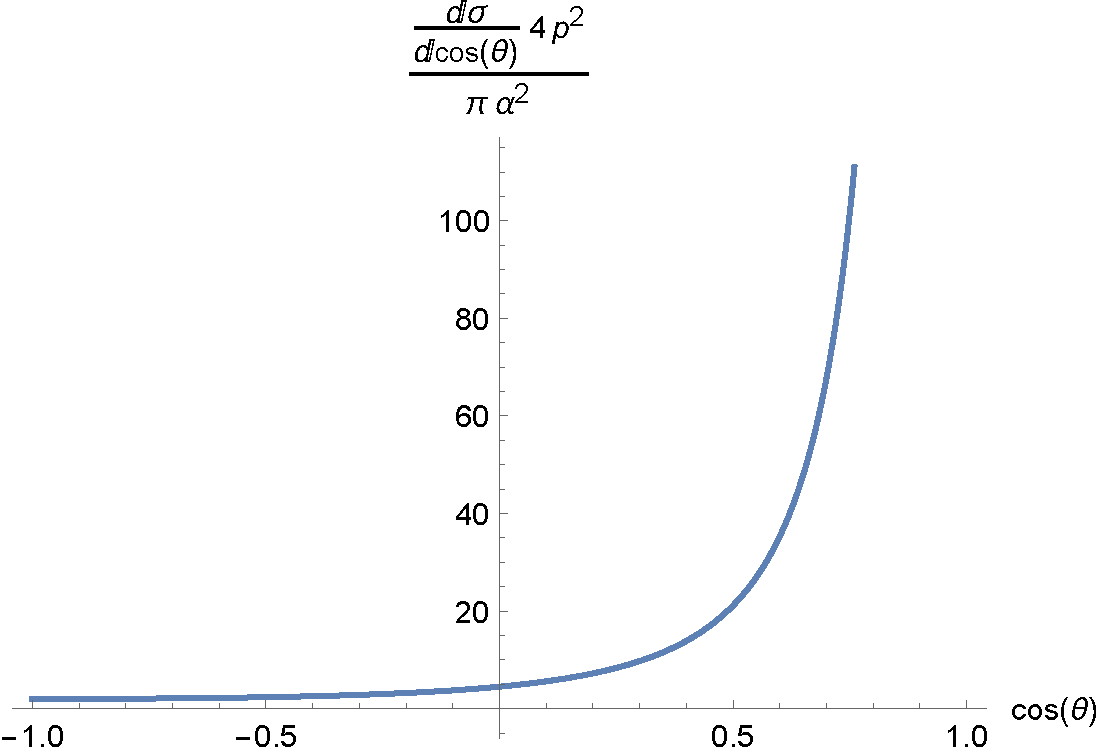
\includegraphics[width=0.6\textwidth]{plot-cross-section.pdf}
    \caption{Plot of \eqref{eq:3-cross-section-cos}}
    \label{fig:cross-section-cos}
\end{figure}

The graph of \eqref{eq:3-cross-section-cos} is \prettyref{fig:cross-section-cos}. It can be seen that the 
cross section diverges as $\theta \to 0$. This traces back to the presence of $t$ in the denominator, which 
is zero when $\theta = 0$, and the $1 / t$ factor itself traces back to the diagram \eqref{eq:t-channel}. 
When $\theta \to 0$, or in other words there is almost no scattering at all, the photon propagator in 
\eqref{eq:t-channel} diverges.

\end{document}